%%% Yili Hong (hong@asu.edu)

\documentclass[paper=letter,fontsize=10pt]{scrartcl} % KOMA-article class

\usepackage[english]{babel}
\usepackage[utf8x]{inputenc}
\usepackage[protrusion=true,expansion=true]{microtype}
\usepackage{amsmath,amsfonts,amsthm}     % Math packages
\usepackage{graphicx}                    % Enable pdflatex
\usepackage[dvipsnames]{xcolor}            % Colors by their 'svgnames'
\usepackage{geometry}
% \usepackage{epstopdf}
	%\textheight=700px                    % Saving trees ;-)
%\usepackage{url}

\usepackage[colorlinks=true,
linkcolor=black,
urlcolor=black]{hyperref} % Color options: https://en.wikibooks.org/wiki/LaTeX/Colors
\usepackage{float}
% \usepackage{etaremune} % reverse enumerate
\usepackage{enumerate}

% \usepackage{wrapfig}
% \usepackage{attachfile}
\usepackage{textcomp}
\usepackage{fontawesome}
\usepackage{lmodern}
% \usepackage{fourier}
\usepackage[T1]{fontenc}
\usepackage{soul} % \ul will make underline work properly spanning multiple lines
\usepackage{lastpage}
\pagenumbering{arabic}
% \pagestyle{empty}           % No pagenumbers/headers/footers


\frenchspacing              % Better looking spacings after periods

%\addtolength{\voffset}{-40pt}
%\addtolength{\textheight}{20pt}

\setlength\topmargin{0pt}
\addtolength\topmargin{-\headheight}
\addtolength\topmargin{-\headsep}
\setlength\oddsidemargin{0pt}
\setlength\textwidth{\paperwidth}
\addtolength\textwidth{-2in}
\setlength\textheight{\paperheight}
%\addtolength\textheight{-3in}
\addtolength\textheight{-2in}
\usepackage{layout}
\usepackage{anyfontsize}
\usepackage{bold-extra}

%%% Custom sectioning}{sectsty package)
%%% ------------------------------------------------------------
\usepackage{sectsty}

\sectionfont{%			            % Change font of \section command
	% \Large \usefont{T1}{put}{m}{n}%		% bch-b-n: Utopia-Bold font
	% \fontsize{15}{16} \usefont{T1}{LinuxBiolinumT-OsF}{b}{sc}%		% bch-b-n: Utopia-Bold font
	\fontsize{14}{16} \usefont{T1}{lmr}{m}{sc}%		% bch-b-n: Utopia-Bold font
	\sectionrule{0pt}{0pt}{-5pt}{0.5pt}}

%%% Macros
%%% ------------------------------------------------------------
\newlength{\spacebox}
\settowidth{\spacebox}{8888888888}			% Box to align text
\newcommand{\sepspace}{\vspace*{1em}}		% Vertical space macro

\newcommand{\MyName}[1]{ % Name
		\LARGE \usefont{T1}{lmr}{m}{sc} #1 % LinuxBiolinumT-OsF
		\par \normalsize \fontshape{sc}}



\newcommand{\MySlogan}[1]{ % Slogan}{optional)
		\small \usefont{T1}{lmtt}{m}{n}\hfill #1
		\par \normalsize \normalfont}

\newcommand{\NewPart}[2]{\section*{{#1} #2}}

\newcommand{\PersonalEntry}[2]{
		\noindent\hangindent=2em\hangafter=0 % Indentation
		\parbox{\spacebox}{        % Box to align text
		\textit{#1}}		       % Entry name}{birth, address, etc.)
		\hspace{1.5em} #2 \par}    % Entry value

\newcommand{\SkillsEntry}[2]{      % Same as \PersonalEntry
		\noindent\hangindent=2em\hangafter=0 % Indentation
		\parbox{\spacebox}{        % Box to align text
		\textit{#1}}			   % Entry name}{birth, address, etc.)
		\hspace{1.5em} #2 \par}    % Entry value

\newcommand{\EducationEntry}[4]{
		\noindent \textbf{#1} \hfill      % Study
		\colorbox{White}{%
			\parbox{6em}{%
			\hfill\color{Black}#2}} \par  % Duration
		\noindent \textit{#3} \par        % School
		\noindent\hangindent=2em\hangafter=0 \small #4 % Description
		\normalsize \par}


\newcommand{\WorkEntry}[5]{				  % Same as \EducationEntry
		\noindent \textbf{#1} \hfill      % Jobname
		\colorbox{White}{%
			\parbox{6em}{%
			\hfill\color{Black}#2}} \par  % Duration
		\noindent \textit{#3,} #4 \par              % Company
		\noindent\hangindent=2em\hangafter=0 \small #5 % Description
		\normalsize \par}

% \newcommand{\PaperEntry}[7]{
% 		\noindent #1, ``\href{#7}{#2}", \textit{#3} \textbf{#4}, #5 (#6).}
\newcommand{\PaperEntry}[6]{
		% \noindent #1 (#2) ``\href{#6}{#3},'' \textit{\ul{#4}}, #5.} % underline the journal title
		\noindent #1 (#2) ``\href{#6}{#3},'' \textit{#4}, #5.} % journal title no underline

\newcommand{\ReviewEntry}[5]{
		\noindent #1 (#2) ``#3,'' \textit{\ul{#4}}, #5.}

\newcommand{\WPEntry}[5]{
        \noindent #1 (#2) ``#3,'' \textit{\ul{#4}}. #5}

\newcommand{\ConfEntry}[6]{
		\noindent #1 (#2) ``#3,'' \textit{#4}, #5. \textcolor{blue}{#6}}

\newcommand{\BookEntry}[4]{
		\noindent #1, ``\href{#3}{#4},'' \textit{#3}.}

\newcommand{\FundingEntry}[5]{
        \noindent #1, ``#2,'' \$#3 (#4, #5).}

\newcommand{\TalkEntry}[3]{
		\noindent #1, #2 #3}

\newcommand{\ThesisEntry}[4]{
		\noindent #1 -- #2, #3,  \textit{#4}}

\newcommand{\CourseEntry}[4]{
		\noindent \item{#1: \ul{#2} #3 #4}}

% \newcommand{\Hong}{\textbf{Hong Y}}
\newcommand{\Hong}{Hong Y}


%%% Begin Document
%%% ------------------------------------------------------------
\begin{document}

%\layout

% you can upload a photo and include it here...
% \begin{wrapfigure}{l}{0.5\textwidth}
% 	\vspace*{-2em}
% 		\includegraphics[width=0.2\textwidth]{Kevin.JPG}
% \end{wrapfigure}
\begin{flushright}
\MyName{Kevin Yili Hong}
\end{flushright}
\MySlogan{\vspace{-0.5in}
\begin{flushright}~\\\faMapMarker~BAC 636, 300 E Lemon St., Tempe, AZ 85287 \\
\faEnvelope~hong@asu.edu~$\cdot$~\href{https://www.linkedin.com/in/yilihong/}{\faLinkedinSquare~yilihong}~$\cdot$~\faPhone~(480)727-4003~
\href{http://kevinhong.me}{\faInternetExplorer~kevinhong.me}
\end{flushright}}


\NewPart{BIO}{}
\bigskip

Yili (Kevin) Hong is an Associate Professor, Co-Director of the Digital Society Initiative, and the Director of Ph.D. Program in the Department of Information Systems at the W. P. Carey School of Business of Arizona State University. Kevin obtained his Ph.D. in Management Information Systems at the Fox School of Business, Temple University. He is currently an Associate Editor at \emph{Information Systems Research} and the \emph{Journal of the Association for Information Systems}. He is also an associate editor for the \emph{ISR} special issues on “Future of Work, Organizations, and Society” and “Market Design and Analytics.”
\bigskip

Kevin’s research interests are in the areas of Digital Platforms, Sharing Economy, Human-AI Interactions, and Smart Health. His research has been published in premier journals such as \emph{Management Science}, \emph{Information Systems Research}, \emph{MIS Quarterly}, \emph{Journal of Management Information Systems}, \emph{Journal of the Association for Information Systems}, and the \emph{Journal of Consumer Psychology}. Kevin’s work has been supported by multiple prestigious grants, from the \emph{National Science Foundation} (2018-2020), the \emph{Robert Wood Johnson Foundation} (2017-2020), the \emph{NET Institute} (2013, 2014, 2015, 2016, 2017, 2018), as well as the \emph{Department of Education} (2011, 2013, 2015).
\bigskip

Kevin's research on online labor markets and gig economy was awarded ACM SIGMIS Best Dissertation Award (2014) and runner-up INFORMS ISS Nunamaker-Chen Dissertation Award (2014). His research papers have received numerous best paper awards at major conferences, including the Workshop on Information Systems and Economics (2018), International Conference on Information Systems (2012, 2018), Hawaii International Conference on System Sciences (2017), America’s Conference on Information Systems (2012), and the China Summer Workshop on Information Management (2018). In 2017, Kevin was awarded the college-wide W. P. Carey Faculty Research Award; Kevin was awarded the AIS Early Career Award (2018) and INFORMS Information Systems Society Early Career Award (2019), respectively. And Kevin was awarded the Best Associate Editor of \emph{Information Systems Research} for 2018. According to the \href{https://www.aisresearchrankings.org/rankings/}{AIS Research Rankings}, Kevin was ranked \#3 based on publications in the Top 4 Information Systems Journals (\emph{MISQ}, \emph{ISR}, \emph{JMIS}, \emph{JAIS}) and \#7 based on the Top 2 Information Systems journals (\emph{MISQ}, \emph{ISR}) for the past 3 years (2016-2018).
\bigskip

At W. P. Carey School of Business, Kevin has taught and led the curriculum development at both the undergraduate (CIS and BDA) and graduate (MS-BA and PhD) levels. Notably, he led the initiative in designing and implementing the new undergraduate college-level analytics core course -- Problem Solving and Actionable Analytics (WPC300). And most recently, he serves as the course coordinator for WPC300, overseeing over 40 sections of the course each year taught by instructors from multiple departments. Further, he led a team of analytics faculty in designing and implementing the core college analytics course in the online and hybrid (onsite + online) formats. Here is a \href{https://player.theplatform.com/p/U8-EDC/dKzF6F2_w14a/select/media/dCsGzS1z_uCq?form=html}{\textcolor{RoyalBlue}{live stream recording}} of Kevin talking about analytics teaching and research in the W. P. Carey "Back-to-Class" Alumni event in April 2019. He received Department of Information Systems' Outstanding Teaching Award in 2016, and was a finalist for the W. P. Carey Huizingh Undergraduate Teaching Award in 2019.
\bigskip

Prior to his academic career, Kevin has worked at China International Capital Corporation (CICC), a large investment bank in China. Besides research and teaching as a faculty member, Kevin serves as an advisor or external research scientist for a number of companies, including Lyft, Freelancer, Magene, Meishijie, Summer, PetSmart, fits.me, Yamibuy, Ports America, and Picmonic.
\newpage
%%% Work experienceearly
%%% ------------------------------------------------------------
\NewPart{Employment}{}
\EducationEntry{Associate Professor of Information Systems \textmd{(with tenure)}}{2018--$\qquad$}{W. P. Carey School of Business, Arizona State University}{}
\EducationEntry{Assistant Professor of Information Systems}{2014--2018}{W. P. Carey School of Business, Arizona State University}{}
\EducationEntry{Director of the IS PhD Program}{2017--$\qquad$}{W. P. Carey School of Business, Arizona State University}{}
% \sepspace
\EducationEntry{Co-Director of the Digital Society Initiative}{2016--$\qquad$}{W. P. Carey School of Business, Arizona State University}{}
\EducationEntry{Instructor and Research Assistant}{2009--2014}{Fox School of Business, Temple University}{}
\EducationEntry{Analyst}{2008--2009}{China International Capital Corporation (CICC), Beijing Office}{}
\EducationEntry{Language Specialist}{2008}{The 29th International Olympic Games}{}


%%% Education
%%% ------------------------------------------------------------
\NewPart{Education}{}

\EducationEntry{PhD Business Administration}{2009--2014}{Fox School of Business, Temple University}{\begin{itemize}
\item[\faCaretRight]{Thesis: ``Three Essays on Global Online Labor Markets for IT Services'' (Advisor: Paul A. Pavlou)}
\item{\href{https://aisnet.org/general/custom.asp?page=ICISSIGMIS}{ACM SIGMIS Doctoral Dissertation Award}}
\item{INFORMS ISS Nunamaker-Chen Dissertation Award}
\item{Best Dissertation Award, Temple University}\end{itemize}}
\vspace{6px}

\EducationEntry{BS Management}{2005--2009}{School of Business, Beijing Foreign Studies University}{\begin{itemize}
\item[\faCaretRight]{Thesis: ``Modeling the Success of Small and Medium Sized Online Vendors in China'' (Advisor: Shan Wang)}
\item Outstanding Graduate\end{itemize}}

\vspace{6px}
\EducationEntry{BA English}{2005--2009}{School of Business, Beijing Foreign Studies University}{} %\faGraduationCap~

\newpage

\NewPart{Research Interests}{}
\textit{Design and Evaluation of IT-based Markets and Business Models}
\begin{itemize}
\item{Digital Economy, Digital Platforms, Online Markets, Auctions, FinTech, Open Innovation}
\end{itemize}
\textit{Societal Impact of Information Technology}
\begin{itemize}
\item{Sharing Economy, Gig Economy, IT Labor, Labor Economics}
\end{itemize}
\textit{Human-AI Interaction and Analytics}
\begin{itemize}
\item{Human-AI Interaction, Smart Health, Social Media Analytics, Recommender Systems, Machine Learning}
\end{itemize}

\NewPart{Editorial Board}{}
\begin{itemize}
\item Associate Editor, \emph{Information Systems Research} (2018--)
\item Associate Editor, \emph{Journal of the Association for Information Systems} (2019--)
\item Associate Editor, \emph{Information Systems Research, Special Issue on ``Humans, Algorithms, and Augmented Intelligence: The Future of Work, Organizations and Society''}
\item Associate Editor, \emph{Information Systems Research, Special Issue on ``Market Design and Analytics''}
\item Associate Editor, \emph{Electronic Commerce Research and Applications} (2017--)
\item Associate Editor, \emph{Electronic Commerce Research} (2018--)
\item Editorial Board, \emph{Journal of the Association for Information Systems} (2017--)
\item Editorial Board, \emph{Journal of the Association for Information Systems} Special Issue on ``Addressing Societal Challenges through Analytics''
\end{itemize}



%%% Awards
%%% ------------------------------------------------------------

\NewPart{Professional Awards}{}
\begin{itemize}
\item 2019 Best Associate Editor of the Year Award, Information Systems Research (ISR)
\item 2019 Nominated for the ASU Outstanding Doctoral Mentor
\item 2019 Best Paper Nomination, Conference on Information Systems and Technology (CIST)
\item 2019 Sandy Slaughter Early Career Award, INFORMS Information Systems Society (ISS)
\item 2019 Finalist, Huizing Undergraduate Teaching Award
\item 2018 Best Paper Award, Workshop on Information Systems and Economics
\item 2018 Best Conference Theme Paper (runner up), International Conference on Information Systems
\item 2018 Best Paper Nomination ($\times2$), International Conference on Information Systems
\item 2018 AIS Early Career Award, Association for Information Systems (AIS)
\item 2018 Best Paper Award, The 12th China Summer Workshop on Information Management
\item 2018 Best Paper Nomination, Pacific Asia Conference on Information Systems
% \item 2018 National Science Foundation Grant %[\faCaretRight
\item 2017 Management Science Meritorious Service Award
\item 2017 W. P. Carey Faculty Research Award
% \item 2017 Robert Wood Johnson Foundation Pioneering Ideas ``Future of Work'' Grant Award
\item 2017 Best Paper Award, Hawaii International Conference on System Sciences
\item 2016 Outstanding Teaching Award, Department of Information Systems (ASU)
\item 2014 Best Paper Nomination, International Conference on Information Systems
\item 2014 ACM SIGMIS Doctoral Dissertation Award, AIS and Association for Computing Machinery
\item 2014 Nunamaker-Chen Dissertation Award (runner up), INFORMS Information Systems Society
\item 2014 Best Dissertation Award, Fox School of Business, Temple University
\item 2014 Dean's Outstanding Publication Award, Fox School of Business, Temple University
\item 2014 Doctoral Consortium Fellow, International Conference on Information Systems
\item 2013 Distinguished Award for Excellence in Teaching, Temple University
\item 2013 Harry A. Cochran Award for Research Excellence
\item 2013 Best Dissertation Proposal Award, Fox School of Business, Temple University
\item 2013 Lynne A. Cronfield Foundation Research Award
\item 2012 Best Conference Paper (runner up), International Conference on Information Systems
\item 2012 Best Conference Paper (runner up), America's Conference on Information Systems
\item 2009 Outstanding Graduate, Beijing Foreign Studies University
\item 2008 Outstanding Language Specialist, International Olympics Committee
\end{itemize}


%%% Major Editorial Board
%%% ------------------------------------------------------------



%%% Premier Journal Papers (UTD, FT)
%%% ------------------------------------------------------------
\NewPart{Premier Journal Publications}{}
%{\href{https://scholar.google.com/citations?user=VwQmUFQAAAAJ}{[Google Scholar]}}

\begin{enumerate}

\item \PaperEntry{Huang N, Burtch G, \Hong, Pavlou PA}{2019}{Unemployment and Worker Participation in the Gig Economy: Evidence from An Online Labor Market}{Information Systems Research}{Forthcoming}{https://papers.ssrn.com/sol3/papers.cfm?abstract_id=3105090}

\item \PaperEntry{Hu Y, Xu A, \Hong, Gal D, Sinha V, Akkiraju R}{2019}{Generating Business Intelligence Through Social Media Analytics: Measuring Brand Personality with Consumer-, Employee-, and Firm-Generated Content}{Journal of Management Information Systems}{36(3):893--930}{https://www.tandfonline.com/doi/full/10.1080/07421222.2019.1628908}

\item \PaperEntry{Huang N, Burtch G, Gu B, \Hong, Liang C, Wang K, Fu D, Yang B}{2019}{Motivating User-Generated Content with Performance Feedback: Evidence from Randomized Field Experiments}{Management Science}{65(1):327--345}{https://pubsonline.informs.org/doi/abs/10.1287/mnsc.2017.2944}

\item \PaperEntry{Kuang L, Huang N, \Hong, Yan Z}{2019}{Spillover Effects of Financial Incentives on User Engagement: Evidence From an Online Knowledge Exchange Platform}{Journal of Management Information Systems}{36(1):289--320}{https://www.tandfonline.com/doi/full/10.1080/07421222.2018.1550564}

\item \PaperEntry{Kanat I, \Hong, Raghu TS}{2018}{Surviving in Global Online Labor Markets for IT Services: A Geo-economic Analysis}{Information Systems Research}{29(4):893–-909}{https://pubsonline.informs.org/doi/abs/10.1287/isre.2017.0751}

\item \PaperEntry{Chen PY, \Hong, Liu Y}{2018}{The Value of Multi-dimensional Rating Systems: Evidence from a Natural Experiment and Randomized Experiments}{Management Science}{64(10):4629--4647}{http://pubsonline.informs.org/doi/abs/10.1287/mnsc.2017.2852}

\item \PaperEntry{Gong J, \Hong, Zentner A}{2018}{Role of Monetary Incentives in the Digital and Physical Inter-Border Labor Flows}{Journal of Management Information Systems}{35(3):866--899}{https://www.tandfonline.com/doi/abs/10.1080/07421222.2018.1481661}

\item \PaperEntry{\Hong, Hu Y, Burtch G}{2018}{Embeddedness, Pro-Sociality, and Social Influence: Evidence from Online Crowdfunding}{MIS Quarterly}{42(4):1211--1224}{https://papers.ssrn.com/sol3/papers.cfm?abstract_id=3125936}

\item \PaperEntry{Burtch G, \Hong, Bapna R, Griskevicius V}{2018}{Stimulating Online Reviews by Combining Financial Incentives and Social Norms}{Management Science}{64(5):2065--2082}{http://pubsonline.informs.org/doi/abs/10.1287/mnsc.2016.2715}

\item \PaperEntry{Burtch G, \Hong, Liu D}{2018}{The Role of Provision Points in Online Crowdfunding}{Journal of Management Information Systems}{35(1):117--144}{https://www.tandfonline.com/doi/full/10.1080/07421222.2018.1440764}

\item \PaperEntry{Huang N, \Hong, Burtch G}{2017}{Social Network Integration and User Content Generation: Evidence from Natural Experiments}{MIS Quarterly}{41(4):1035--1058 (Lead Article)}{https://misq.org/social-network-integration-and-user-content-generation-evidence-from-natural-experiments.html}

\item \PaperEntry{\Hong, Pavlou PA}{2017}{On Buyer Selection of Service Providers in Online Outsourcing Platforms for IT Services}{Information Systems Research}{28(3):547--562}{http://pubsonline.informs.org/doi/abs/10.1287/isre.2017.0709}

\item \PaperEntry{\Hong, Pavlou PA, Shi N, Wang K}{2016}{On the Role of Fairness and Social Distance in Designing Effective Social Referral Systems}{MIS Quarterly}{41(3):787--809}{https://misq.org/on-the-role-of-fairness-and-social-distance-in-designing-effective-social-referral-systems.html}

\item \PaperEntry{\Hong, Huang N, Burtch G, Li C}{2016}{Culture, Conformity and Emotional Suppression in Online Reviews}{Journal of the Association for Information Systems}{17(11):308--329}{http://aisel.aisnet.org/jais/vol17/iss11/2/}

\item \PaperEntry{Huang N, Burtch G, \Hong, Polman E}{2016}{Effects of Multiple Psychological Distances on Construal and Consumer Evaluation: A Field Study of Online Reviews}{Journal of Consumer Psychology}{26(4):474--482}{https://doi.org/10.1016/j.jcps.2016.03.001}

\item \PaperEntry{\Hong, Wang CA, Pavlou PA}{2016}{Comparing Open and Sealed Bid Auctions: Evidence from Online Labor Markets}{Information Systems Research}{27(1):49--69}{https://doi.org/10.1287/isre.2015.0606}

\item \PaperEntry{\Hong, Pavlou PA}{2014}{Product Fit Uncertainty in Online Markets: Nature, Effects, and Antecedents}{Information Systems Research}{25(2):328--344}{https://doi.org/10.1287/isre.2014.0520}

\item \PaperEntry{Dimoka A, \Hong, Pavlou PA}{2012}{On Product Uncertainty in Online Markets: Theory and Evidence}{MIS Quarterly}{36(2):395--426}{https://misq.org/on-product-uncertainty-in-online-markets-theory-and-evidence.html}

\end{enumerate}



%%% Other Publications
%%% ------------------------------------------------------------

\NewPart{Other Publications}{}

\begin{enumerate}
\item \PaperEntry{Fu D, \Hong, Wang K, Fan W}{2018}{Effects of Membership Tier on User Content Generation Behavior in an Online Marketplace}{Electronic Commerce Research}{18(3):457--483}{https://link.springer.com/article/10.1007/s10660-017-9266-7}

\item \PaperEntry{\Hong, Pavlou PA}{2011}{Online Labor Markets: An Informal Freelancer Economy}{IBIT Report}{Fall 2011}{https://papers.ssrn.com/sol3/papers.cfm?abstract_id=2132869}

\item \PaperEntry{Wang S, \Hong, Archer N, Wang Y}{2011}{Modeling the Success of Small and Medium Sized Online Vendors in Business to Business Electronic Marketplaces in China: A Motivation--Capability Framework}{Journal of Global Information Management}{19(4):45--75}{https://www.igi-global.com/article/modeling-success-small-medium-sized/58551}

\end{enumerate}


%%% Papers Under Review
%%% ------------------------------------------------------------

\NewPart{Papers Under Review}{}
\begin{enumerate}

\item \ReviewEntry{\Hong, Chen PY, Hitt LM, Wu SY}{2019}{Measuring Product Type Using Online Review Variance}{\protect\newline Information Systems Research}{R\&R, Prepare for 4th round review}{}

\item \ReviewEntry{Zheng X, Ren XY, \Hong, Cao JS, Yang S}{2019}{The Impact of Variances in Multi-Dimensional Rating Systems on the Sales of High-Involvement Products: A Multi-Method Study}{\protect\newline MIS Quarterly}{R\&R, Prepare for 3rd round review}{}

\item \ReviewEntry{Liu Q, Du Q, \Hong, Fan W}{2019}{User Idea Implementation in Open Innovation Communities: An Elaboration Likelihood Model Perspective}{\protect\newline Information Systems Journal}{R\&R, Prepare for 3rd round review}{}

\item \ReviewEntry{Liang C, \Hong, Gu B}{2019}{IT-enabled Monitoring and Labor Contracting in Online Platforms: Evidence from a Natural Experiment}{\protect\newline Information Systems Research}{R\&R, under 2nd round review}{}

\item \ReviewEntry{Li Z, \Hong, Zhang Z}{2019}{How Do On-demand Ride-sharing Services Affect Traffic Congestion?}{\protect\newline MIS Quarterly}{R\&R, Under 2nd round review}{}

\item \ReviewEntry{Hu Y, \Hong}{2019}{Event Detection and Recommendation using Social Media for Promoting Civic Awareness and Engagement for Local Communities}{\protect\newline INFORMS Journal on Computing}{R\&R, Prepare for 2nd round review}{}

\item \ReviewEntry{\Hong, Shao BBM}{2019}{Effectiveness of Experience in E-Procurement: Roles of Temporal Distance and Task Routinization}{\protect\newline Production and Operations Management}{R\&R, Prepare for 2nd round review}{}

\item \ReviewEntry{\Hong, Peng J, Burtch G, Huang N}{2019}{Do You Have Time for a Quick Chat? Direct Messaging System Usage and Hiring Outcomes in Online Labor Markets}{\protect\newline Information Systems Research}{R\&R, prepare for 2nd round review}{}

\item \ReviewEntry{Zheng Z, \Hong, Pavlou PA}{2019}{Bid Price Dispersion in the Contracting of Online Service Procurement Auctions}{\protect\newline Production and Operations Management}{R\&R, Prepare for 2nd round review}{}

\item \ReviewEntry{Li Z, \Hong, Zhang Z}{2019}{The Empowering and Spillover Effects of the Platform-based Sharing Economy on the Labor Market}{\protect\newline Journal of Management Information Systems}{R\&R, prepare for 2nd round review}{}

\item \ReviewEntry{Zhao K, Hu Y, \Hong, Westland C}{2019}{Understanding Factors that Influence User Popularity in Live Streaming Platforms}{\protect\newline Journal of the Association for Information Systems}{R\&R, Prepare for 2nd round review}{}

\item \ReviewEntry{Cheng C, Hu Y, Lu Y, \Hong}{2019}{Everyone Can Be a Star in the Digital Economy: Quantifying the Business Value of Live Streaming Technology in Online Retail}{\protect\newline Information Systems Research}{Under 1st round review}{}

\item \ReviewEntry{Burtch G, \Hong, Kumar S}{2019}{The Contingent Complementary Benefits of Dispute Resolution and Online Reputation Systems}{\protect\newline Production and Operations Management}{Under 1st round review}{}

\item \ReviewEntry{Burtch G, He Q, \Hong, Lee D}{2019}{The Role of Peer Awards on User Creativity: Evidence from a Randomized Field Experiment}{\protect\newline Management Science}{Under 1st round review}{}

% \item \ReviewEntry{Liang C, \Hong, Gu B}{2019}{Home Bias in Online Employment: Evidence from an Online Labor Market}{\protect\newline Management Science}{Under 1st round review}{}

\item \ReviewEntry{\Hong, Chen PY, Shao BBM, Liang C}{2019}{The Role of Auction Parameters in Online Outsourcing Platforms for Service Procurement}{\protect\newline Journal of Operations Management}{Under 1st round review}{}

\item \ReviewEntry{He Q, Benjamin V, \Hong, Raghu TS}{2018}{Multi-channel Complementarity in Goal-directed Platforms}{\protect\newline MIS Quarterly}{Reject and resubmit}{}


\item \ReviewEntry{Li J, Ge Y, \Hong, Cheema A, Gu B}{2018}{Textual Review Dimensionality And Helpfulness: A Multi-Method Study}{\protect\newline Information Systems Research}{Reject and resubmit}{}

\end{enumerate}


%%% Working Papers with drafts
%%% ------------------------------------------------------------

\NewPart{Working Papers}{\small\textmd{(Completed Drafts Available)}} % with the option of \textnormal
\begin{enumerate}

\item \WPEntry{He Y, \Hong, Huang N, Xu X}{2019}{Engineering Demand Information in the Presence of Capacity Constraints: A Large-Scale Randomized Field Experiment on a Matching Platform}{\protect\newline Target: ISR Special Issue on Market Design and Analytics}{}{}

\item \WPEntry{Zhao K, Hu Y, Lu Y, \Hong}{2019}{Examining the Content Switching and Competition of Live Streamers from the Audience Viewing Choices}{\protect\newline Target: Information Systems Research}{}{}

\item \WPEntry{Liang C, Peng J, \Hong, Gu B, Peng J}{2019}{Economic Costs of Monitoring}{\protect\newline Target: Management Science}{}{}

\item \WPEntry{Huang N, Chen PY, \Hong, Wu SY}{2019}{Conspicuous Social Sharing: Evidence from A Randomized Field Experiment}{\protect\newline Target: Management Science}{}{}

\item \WPEntry{Sabzehzar A, Butch G, \Hong, Raghu TS}{2019}{The Role of Religion in Prosocial Lending}{\protect\newline Target: MIS Quarterly}{}{}

\item \WPEntry{Hou J, Huang N, \Hong, Chen P}{2018}{Free or Costly Bidding? A Quasi-Natural Experiment in Large-scale Online Procurement Auctions}{\protect\newline Target: Production and Operations Management}{}{}

\item \WPEntry{Liang C, \Hong, Gu B}{2019}{Why Gender Wage Gap does not Necessarily Mean Gender Bias? Evidence from Online Gig Economy}{\protect\newline Target: Management Science}{}{}

\item \ReviewEntry{Liu Q, Du Q, \Hong, Fan W}{2018}{Predicting Open Innovation Idea Selection from Content Features}{\protect\newline Target: Information Systems Research}{}{}

\item \ReviewEntry{Sabzehzar A, \Hong, Raghu TS}{2019}{Dynamic Shifting in Prosocial Lending Priorities: Evidence from a Natural Experiment}{\protect\newline Target: PNAS}{}{}

\item \WPEntry{He Q, Benjamin V, \Hong, Raghu TS}{2018}{Role of Reference Points in the Goal-directed Platform: A Randomized Field Experiment}{\protect\newline Target: Journal of Marketing Research}{}{}

\item \WPEntry{Liu Y, Chen PY, \Hong, Ge Y}{2018}{The Impact of Rating System Design on Opinion Sharing}{\protect\newline Target: Information Systems Research}{}{}

\item \WPEntry{Kanat I, \Hong, Gu B, Raghu TS}{2018}{An Empirical Study of Add-on Content and User Engagement}{\protect\newline Target: MIS Quarterly}{}{}

\item \WPEntry{Hu Y, \Hong}{2018}{Analyzing Location Disclosure Behaviors on Instagram}{\protect\newline Target: MIS Quarterly}{}{}

\end{enumerate}
%\newpage


%%% Grants
%%% ------------------------------------------------------------

\NewPart{Funding and Grants}{}
\begin{itemize}
\item \FundingEntry {Dean’s Excellence in Research Grant}{Peer Symbolic Awards and User Creativity}{20,000}{PI}{2019}
\item \FundingEntry {Center for the Study of Economic Liberty}{The Role of Religion in Online Platforms}{5,000}{co-PI}{2019}
\item \FundingEntry {NET Institute}{\href{http://www.netinst.org/Chen_18-03.pdf}{Gender Wage Gap in Online Gig Economy and Gender Differences in Job Preferences}}{3,000}{co-PI}{2018}
\item \FundingEntry {Dean’s Excellence in Research Grant}{Private Communication in Online Platforms}{20,000}{PI}{2018}
\item \FundingEntry {National Science Foundation, Decision, Risk and Management Sciences (DRMS)}{\href{https://www.nsf.gov/awardsearch/showAward?AWD_ID=1824432}{Expectation Bias and the Gender Wage Gap in the Online Gig Economy}}{15,914}{co-PI}{2018--2020}
\item \FundingEntry {Center for the Study of Economic Liberty}{Gender Wage Gap does not Equal Gender Bias}{10,000}{co-PI}{2018}
\item \FundingEntry {Amazon Cloud Credits for Research}{Online Labor Markets}{12,200}{co-PI}{2018}
\item \FundingEntry {National Science Foundation of China (NSFC)}{Social Referral Design}{10,000}{co-PI}{05/2017--06/2019}
\item \FundingEntry {NET Institute}{\href{http://www.netinst.org/Liang_17-06.pdf}{Home Bias in Global Employment}}{4,500}{co-PI}{2017}
\item \FundingEntry {Robert Wood Johnson Foundation}{Future of Work Pioneering Grant}{120,024}{PI}{04/2017--01/2020}
\item \FundingEntry {Center for the Study of Economic Liberty}{Sharing Economy and Gig Economy Projects}{6,000}{PI}{2017}
\item \FundingEntry {Google}{Cloud Platform Education Grants}{11,100}{PI}{2016}
\item \FundingEntry {NET Institute}{\href{http://www.netinst.org/Liang_16-01.pdf}{Effects of IT-enabled Monitoring on Labor Contracting in Online Platforms: Evidence from a Natural Experiment}}{4,500}{co-PI}{2016}
\item \FundingEntry {Amazon Cloud Credits for Research}{IT-enabled Monitoring}{5,000}{PI}{2016}
\item \FundingEntry {Department of Education}{CIBER Grant Award}{2,500}{co-PI}{2015}
\item \FundingEntry {NET Institute}{\href{http://www.netinst.org/Huang_Hong_Burtch_15-04.pdf}{Digital Social Visibility, Anonymity and User Content Generation: Evidence from Natural Experiments}}{3,000}{co-PI}{2015}
\item \FundingEntry {NET Institute}{\href{http://www.netinst.org/Hong_14-03.pdf}{Measuring Product Type with Dynamics of Online Product Review Variances: A Theoretical Model and the Empirical Applications}}{3,000}{co-PI}{2014}
\item \FundingEntry {Department of Education}{CIBER Grant Award}{5,000}{PI}{2013}
\item \FundingEntry {NET Institute}{\href{http://www.netinst.org/Hong_Wang_13-05.pdf}{How Does Bid Visibility Matter in Buyer-Determined Auctions? Comparing Open and Sealed Bid Auctions in Online Labor Markets}}{3,000}{PI}{2013}
\item \FundingEntry {Department of Education}{CIBER Grant Award}{5,000}{co-PI}{2010}
%\faBitcoin
\end{itemize}


%%% Conference Papers
%%% ------------------------------------------------------------

\NewPart{Conference Papers}{}
\begin{enumerate}

\item \ConfEntry{Burtch G, He Q, \Hong, Lee D}{2019}{Peer Awards Increase Content Generation but Reduce Content Novelty}{Workshop on Information Systems and Economics (WISE)}{Munich, Germany}{}

\item \ConfEntry{Liang C, Peng J, \Hong, Gu B}{2019}{Economic Cost of Monitoring}{Conference on Digital Experimentation (CODE)}{Cambridge, MA}{}

\item \ConfEntry{Burtch G, He Q, \Hong, Lee D}{2019}{Peer Symbolic Awards Increase User Content Generation but Reduce Content Novelty}{Conference on Digital Experimentation (CODE)}{Cambridge, MA}{}

\item \ConfEntry{Hu Y, \Hong, Peng J, Burtch G, Huang N}{2019}{Promoting Civic Awareness and Engagement for Local Communities via Event Detection and Recommendation on Twitter}{INFORMS Conference on Information Systems and Technology (CIST)}{Seattle, WA}{}

\item \ConfEntry{Liang C, Peng J, \Hong, Gu B}{2019}{Economic Cost of Monitoring}{INFORMS Conference on Information Systems and Technology (CIST)}{Seattle, WA}{\protect\newline Nominated for the Best Paper Award}

\item \ConfEntry{Burtch G, He Q, \Hong, Lee D}{2019}{Peer Symbolic Awards Increase User Content Generation but Reduce Content Novelty}{INFORMS Conference on Information Systems and Technology (CIST)}{Seattle, WA}{}

\item \ConfEntry{Hou J, Huang N, \Hong, Chen P}{2019}{Participation Costs Reduce the Overbidding and Increase Matching Rates in Two-sided Procurement Platforms}{INFORMS Conference on Information Systems and Technology (CIST)}{Seattle, WA}{}

\item \ConfEntry{Burtch G, He Q, \Hong, Lee D}{2019}{Peer Symbolic Awards Increase Content Generation but Reduce Content Novelty}{Proceedings of the International Conference on Information Systems (ICIS)}{Munich, Germany}{}

\item \ConfEntry{\Hong, Peng J, Burtch G, Huang N}{2019}{Pipes versus Prisms: Direct Messaging System and Hiring Outcomes in Online Labor Markets}{Proceedings of the International Conference on Information Systems (ICIS)}{Munich, Germany}{}

\item \ConfEntry{Sabzehzar A, Burtch G, \Hong, Raghu TS}{2019}{The Role of Religion in Online Prosocioal Lending}{Proceedings of the International Conference on Information Systems (ICIS)}{Munich, Germany}{}

\item \ConfEntry{Gu R, \Hong}{2019}{Addressing Health Misinformation Disssemination on Mobile Social Media}{Proceedings of the International Conference on Information Systems (ICIS)}{Munich, Germany}{}

\item \ConfEntry{Burtch G, He Q, \Hong, Lee D}{2019}{Peer Symbolic Awards Increase Content Generation but Reduce Content Novelty}{Statistical Challenges in eCommerce Research (SCECR)}{Hong Kong, China}{}

\item \ConfEntry{Liang C, \Hong, Gu B, Peng J}{2019}{Gender Differences in Job Preferences}{Statistical Challenges in eCommerce Research (SCECR)}{Hong Kong, China}{}

\item \ConfEntry{Burtch G, He Q, \Hong, Lee D}{2019}{Peer Symbolic Awards Increase Content Generation but Reduce Content Novelty}{WEBEIS}{Minneapolis, MN}{}

\item \ConfEntry{Zhao K, Hu Y, Lu Y, \Hong}{2019}{Understanding the Dynamic Competition in Live Streaming Platform}{Winter Conference on Business Analytics (WCBA)}{Snowbird, Utah}{}

\item \ConfEntry{Sabzehzar A, Butch G, \Hong, Raghu TS}{2019}{The Role of Religion in Prosocial Lending}{Winter Conference on Business Analytics (WCBA)}{Snowbird, Utah}{}

\item \ConfEntry{\Hong, Peng J, Burtch G, Huang N}{2018}{Pipes versus Prisms: Direct Messaging System and Hiring Outcomes in Online Labor Markets}{Workshop on Information Systems and Economics (WISE)}{San Francisco, California}{}

\item \ConfEntry{Liang C, \Hong, Gu B, Peng J}{2018}{Gender Differences in Job Preferences}{Workshop on Information Systems and Economics (WISE)}{San Francisco, California}{\protect\newline Winner of the Best Paper Award}

\item \ConfEntry{\Hong, Chen PY, Shao BBM, Liang C}{2018}{Auction Parameters and Bidder Entry: Evidence from Online Outsourcing Platforms}{Workshop on Information Technology and Systems (WITS)}{San Jose, California}{}

\item \ConfEntry{He Q, Benjamin V, \Hong, Raghu TS}{2017}{Role of Reference Points in the Goal-directed Website: A Randomized Field Experiment}{Workshop on Information Technology and Systems (WITS)}{San Jose, California}{}

\item \ConfEntry{Chen C, Hu Y, \Hong, Lu Y}{2018}{Everyone Can Be a Star: Quantifying Grassroots Online Sellers' Live Streaming Effects on Product Sales}{Decision Sciences Institute Annual Conference (DSI)}{Chicago, IL}{}

\item \ConfEntry{Chen C, Hu Y, \Hong, Lu Y}{2018}{Online Streaming and Data Visualization}{Decision Sciences Institute Annual Conference (DSI)}{Chicago, IL}{}

\item \ConfEntry{\Hong, Peng J, Burtch G, Huang N}{2018}{Direct Messaging System and Hiring Outcomes in Online Labor Markets}{Decision Sciences Institute Annual Conference (DSI)}{Chicago, IL}{}

\item \ConfEntry{Liang C, \Hong, Gu B, Peng J}{2018}{Gender Wage Gap in Gig Economy and Gender Differences in Job Preferences}{CODE{@}MIT Conference}{Cambridge, MA}{}

\item \ConfEntry{\Hong, Peng J, Burtch G, Huang N}{2018}{Do You Have Time for a Quick Chat? Direct Messaging System Usage and Hiring Outcomes in Online Labor Markets}{INFORMS Conference on Information Systems and Technology (CIST)}{Phoenix, AZ}{}

\item \ConfEntry{Liang C, \Hong, Gu B, Peng J}{2018}{Gender Wage Gap in Gig Economy and Gender Differences in Job Preferences}{INFORMS Conference on Information Systems and Technology (CIST)}{Phoenix, AZ}{}

\item \ConfEntry{Huang N, Burtch G, \Hong, Pavlou P}{2018}{Local Economic Conditions and Worker Participation in the Online Gig Economy}{INFORMS Conference on Information Systems and Technology (CIST)}{Phoenix, AZ}{}

\item \ConfEntry{Chen C, Hu Y, \Hong, Lu Y}{2018}{Everyone Can Be a Star: Quantifying Grassroots Online Sellers' Live Streaming Effects on Product Sales}{INFORMS Conference on Information Systems and Technology (CIST)}{Phoenix, AZ}{}

\item \ConfEntry{Chen C, Hu Y, \Hong, Lu Y}{2018}{Everyone Can Be a Star: Quantifying Grassroots Online Sellers' Live Streaming Effects on Product Sales}{INFORMS Data Science Conference}{Phoenix, AZ}{}

\item \ConfEntry{Zhao K, Hu Y, Lu Y, \Hong}{2018}{Change, We Can Believe in: Examining Spillover Effect of Content Switch on Live Streaming Platform}{INFORMS Data Science Conference}{Phoenix, AZ}{}

\item \ConfEntry{Hu Y, \Hong, Gal D, Xu A, Sinha V, Akkiraju R}{2018}{Modeling Brand Personality with Business Value of Social Media Analytics: Predicting Brand Personality with User-generated Content and Firm-generated Content}{INFORMS Data Science Conference}{Phoenix, AZ}{}

\item \ConfEntry{Chen C, Hu Y, \Hong, Lu Y}{2018}{Everyone Can Be a Star: Quantifying Grassroots Online Sellers' Live Streaming Effects on Product Sales}{Proceedings of the International Conference on Information Systems (ICIS)}{San Francisco, CA}{}

\item \ConfEntry{Zhao K, Hu Y, Lu Y, \Hong}{2018}{Change, We Can Believe in: Examining Spillover Effect of Content Switch on Live Streaming Platform}{Proceedings of the International Conference on Information Systems (ICIS)}{San Francisco, CA}{}

\item \ConfEntry{Hu Y, \Hong, Gal D, Xu A, Sinha V, Akkiraju R}{2018}{Modeling Brand Personality with Business Value of Social Media Analytics: Predicting Brand Personality with User-generated Content and Firm-generated Content}{Proceedings of the International Conference on Information Systems (ICIS)}{San Francisco, CA}{}

\item \ConfEntry{Li Z, \Hong, Zhang Z}{2018}{Empowerment or Substitution? Entry of Platform-based Sharing Economy on the Local Labor Markets}{Proceedings of the International Conference on Information Systems (ICIS)}{San Francisco, CA}{}

\item \ConfEntry{Liu Q, Du Q, \Hong, Fan W}{2018}{What Kind of User-Generated Ideas Are More Likely to be Implemented? Evidence from an Open Innovation Community }{Proceedings of the International Conference on Information Systems (ICIS)}{San Francisco, CA}{}

\item \ConfEntry{Huang N, Burtch G, \Hong, Pavlou P}{2018}{Local Economic Conditions and Worker Participation in the Online Gig Economy}{Proceedings of the International Conference on Information Systems (ICIS)}{San Francisco, CA}{\protect\newline Nominated for the Best Paper Award}

\item \ConfEntry{Liang C, \Hong, Gu B}{2018}{Gender Wage Gap in Online Gig Economy and Gender Differences in Job Preferences}{Proceedings of the International Conference on Information Systems (ICIS)}{San Francisco, CA}{}

\item \ConfEntry{Zheng X, Ren XY, \Hong, Cao JS, Yang S}{2018}{Information Inconsistencies in Multi-Dimensional Rating Systems}{Proceedings of the International Conference on Information Systems (ICIS)}{San Francisco, CA}{\protect\newline Best Conference Theme Paper Award (runner-up)}

\item \ConfEntry{Liang C, \Hong, Gu B}{2018}{Effects of IT-enabled Monitoring Systems: Evidence from An Online Labor Market}{The Platform Research Symposium}{Boston, MA}{}

\item \ConfEntry{Liang C, \Hong, Gu B}{2018}{Home Bias in Online Employment: Evidence from an Online Labor Market}{The 12th China Summer Workshop on Information Management (CSWIM)}{Qingdao, China}{\protect\newline Winner of the Best Paper Award}

\item \ConfEntry{\Hong, Peng J, Burtch G, Huang N}{2018}{Role of Private Communication in Online Labor Markets}{Statistical Challenges in eCommerce Research (SCECR)}{Rotterdam, Netherlands}{}

\item \ConfEntry{Liang C, \Hong, Gu B}{2018}{Home Bias in Hiring: Evidence from an Online Labor Market}{Pacific Asia Conference on Information Systems (PACIS)}{Yokohama, Japan}{\protect\newline Nominated for the Best Paper Award}

\item \ConfEntry{Liang C, \Hong, Gu B}{2018}{Home Bias in Online Employment: A Quasi-Natural Experiment}{WEBEIS}{Arlington, VA}{}

\item \ConfEntry{\Hong, Peng J, Burtch G, Huang N}{2018}{Role of Communication in Online Platforms}{Americas Conference on Information Systems}{New Orleans, LA}{}

\item \ConfEntry{\Hong, Peng J, Burtch G, Huang N}{2018}{Communication in Online Employment}{POMS 2018 Annual Conference}{Houston, TX}{}

\item \ConfEntry{Hu Y, Zhao K, \Hong}{2018}{Identify and Modeling Players in Live Streaming Community}{POMS 2018 Annual Conference}{Houston, TX}{}

\item \ConfEntry{Huang N, Chen PY, \Hong, Wu SY}{2018}{Digital Nudging for Online Social Sharing: Evidence from A Randomized Field Experiment}{51st Hawaii International Conference on System Sciences (HICSS)}{Hawaii, US}{}

\item \ConfEntry{Liang C, \Hong, Gu B}{2018}{Home Bias in Online Employment}{51st Hawaii International Conference on System Sciences (HICSS)}{Hawaii, US}{}

\item \ConfEntry{Li Z, \Hong, Zhang Z}{2018}{An Empirical Analysis of the Impacts of the Sharing Economy Platforms on the U.S. Labor Market}{51st Hawaii International Conference on System Sciences (HICSS)}{Hawaii, US}{}

\item \ConfEntry{Gong J, \Hong, Zentner A}{2018}{Vanishing Borders in the Internet Age: The Income Elasticity of Virtual versus Physical Migration}{51st Hawaii International Conference on System Sciences (HICSS)}{Hawaii, US}{}

\item \ConfEntry{\Hong, Chen PY, Shao BBM, Liang C}{2018}{Effect of Auction Design on Bidder Entry: Evidence from An Online Labor Market}{51st Hawaii International Conference on System Sciences (HICSS)}{Hawaii, US}{}

\item \ConfEntry{He Q, Benjamin V, \Hong, Raghu TS}{2017}{Multi-Channel Complementarity in the Online Learning Context}{Workshop on Information Technology and Systems (WITS)}{Seoul, South Korea}{}

\item \ConfEntry{Li J, Ge Y, \Hong, Cheema A, Gu B}{2017}{Review Dimensionality and Helpfulness: A Multi-method Study}{Workshop on Information Technology and Systems (WITS)}{Seoul, South Korea}{}

\item \ConfEntry{Liang C, \Hong, Gu B}{2017}{Home Bias in Online Employment}{Workshop on Information Systems and Economics (WISE)}{Seoul, South Korea}{}

\item \ConfEntry{Liang C, \Hong, Gu B}{2017}{Home Bias in Online Employment}{Conference on Information Systems and Technology (CIST)}{Houston, TX}{}

\item \ConfEntry{Liu Y, Chen PY, \Hong, Ge Y}{2017}{The Impact of Rating System Design on Opinion Sharing}{Conference on Information Systems and Technology (CIST)}{Houston, TX}{}

\item \ConfEntry{Li J, Ge Y, \Hong, Cheema A, Gu B}{2017}{Review Dimensionality and Helpfulness: Evidence from a Supervised Topic Modeling, an Empirical Analysis, and a Randomized Experiment}{Conference on Information Systems and Technology (CIST)}{Houston, TX}{}

\item \ConfEntry{Liu Y, Chen PY, \Hong, Ge Y}{2017}{The Impact of Rating System Design on Opinion Sharing}{POMS 2017 Annual Conference}{Seattle, WA}{}

\item \ConfEntry{Liang C, \Hong, Gu B}{2017}{Home Bias in Online Employment}{Proceedings of the International Conference on Information Systems (ICIS)}{Seoul, South Korea}{}

\item \ConfEntry{Liu Y, Chen PY, \Hong, Ge Y}{2017}{The Impact of Rating System Design on Opinion Sharing}{Proceedings of the International Conference on Information Systems (ICIS)}{Seoul, South Korea}{}

\item \ConfEntry{Li J, Ge Y, \Hong, Cheema A, Gu B}{2017}{Review Dimensionality and Helpfulness: Evidence from a Supervised Topic Modeling, an Empirical Analysis, and a Randomized Experiment}{Winter Conference on Business Analytics (WCBA)}{Snowbird, Utah}{}

\item \ConfEntry{Huang N, Gu B, Burtch B, \Hong, Liang C, Wang K, Fu D, Yang B}{2017}{Designing Effective Performance Feedback Notification Systems to Stimulate Content Contribution: Evidence from a Crowdsourcing Recipe Platform}{50th Hawaii International Conference on System Sciences (HICSS)}{Hawaii, US}{\protect\newline Winner of the Best Paper Award}

\item \ConfEntry{Kanat I, \Hong, Gu B, Raghu TS}{2017}{If You Let Them Build It, They Will Stay! An Empirical Study of Add-on Content and User Engagement}{50th Hawaii International Conference on System Sciences (HICSS)}{Hawaii, US}{\protect\newline Nominated for the Best Paper Award}

\item \ConfEntry{Li Z, \Hong, Zhang Z}{2017}{Do Ride Sharing Services Affect Traffic Congestion? An Empirical Study of Uber Entry}{50th Hawaii International Conference on System Sciences (HICSS)}{Hawaii, US}{}

\item \ConfEntry{Hu Y, \Hong}{2017}{Modeling and Predicting Social Media Engagement in Real-World Events}{50th Hawaii International Conference on System Sciences (HICSS)}{Hawaii, US}{\protect\newline Nominated for the Best Paper Award}

\item \ConfEntry{Zheng ZA, \Hong, Pavlou PA}{2016}{Matching in Online Labor Markets for IT Services: Bid Price Dispersion, Buyer Indecision, and Freelancer Regret}{Workshop on Information Systems and Economics (WISE)}{Hawaii, US}{}

\item \ConfEntry{Liang C, \Hong, Gu B}{2016}{Effects of IT-enabled Monitoring Systems: Evidence from Fixed and Time-based Contracts in An Online Labor Market}{Workshop on Information Systems and Economics (WISE)}{Dublin, Ireland}{}

\item \ConfEntry{Huang N, Gu B, Burtch B, \Hong, Liang C, Wang K, Fu D, Yang B}{2016}{Stimulating User-Generated Content via Performance Feedback: A Randomized Mobile Field Experiment}{CODE{@}MIT Conference}{Cambridge, MA}{}

\item \ConfEntry{Li Z, \Hong, Zhang Z}{2016}{Do Ride Sharing Services Affect Traffic Congestion? An Empirical Study of Uber Entry}{INFORMS Annual Meeting}{Nashville, TN}{}

\item \ConfEntry{Liang C, \Hong, Gu B}{2016}{Effects of IT-enabled Monitoring Systems in Online Labor Markets}{Conference on Information Systems and Technology (CIST)}{Nashville, TN}{}

\item \ConfEntry{Huang N, Gu B, Burtch B, \Hong, Liang C, Wang K, Fu D, Yang B}{2016}{Stimulating User-Generated Content via Performance Feedback: A Randomized Mobile Field Experiment}{Conference on Information Systems and Technology (CIST)}{Nashville, TN}{}

\item \ConfEntry{Huang N, Gu B, Burtch B, \Hong, Liang C, Wang K, Fu D, Yang B}{2016}{Stimulating User-Generated Content via Performance Feedback: A Randomized Mobile Field Experiment}{Proceedings of the International Conference on Information Systems (ICIS)}{Dublin, Ireland}{}

\item \ConfEntry{Liang C, \Hong, Gu B}{2016}{Effects of IT-enabled Monitoring Systems in Online Labor Markets}{Proceedings of the International Conference on Information Systems (ICIS)}{Dublin, Ireland}{}

\item \ConfEntry{Li Z, \Hong, Zhang Z}{2016}{Do Ride Sharing Services Affect Traffic Congestion? An Empirical Study of Uber Entry}{Proceedings of the International Conference on Information Systems (ICIS)}{Dublin, Ireland}{}

\item \ConfEntry{Hu Y, \Hong}{2016}{Analyzing Location Disclosure Behavior on Instagram}{Annual International Conference on Computational Social Science}{Evanston, IL}{}

\item \ConfEntry{Huang N, Gu B, Burtch B, \Hong, Liang C}{2016}{Stimulating UGC Contribution via Performance Feedback: A Randomized Mobile Field Experiment}{Statistical Challenges in eCommerce Research (SCECR)}{Naxos, Greece}{}

\item \ConfEntry{Kanat I, \Hong, Raghu TS}{2015}{Surviving and Thriving in Online Labor Markets: A Geoeconomic Analysis}{Workshop on Information Systems and Economics (WISE)}{Dallas, TX}{}

\item \ConfEntry{Burtch G, \Hong, Bapna R, Griskevicius V}{2015}{What Are Social Incentives Worth?}{Proceedings of the International Conference on Information Systems (ICIS)}{Dallas, TX}{}

\item \ConfEntry{\Hong, Hu Y, Burtch G}{2015}{Social Broadcasting or Social Sharing? Understanding the Crowd's Contribution to Public vs. Private Goods in Crowdfunding Campaigns}{Proceedings of the International Conference on Information Systems (ICIS)}{Dallas, TX}{}

\item \ConfEntry{Huang N, \Hong, Burtch G}{2015}{Anonymity and Language Usage: A Natural Experiment of Social Network Integration}{Proceedings of the International Conference on Information Systems (ICIS)}{Dallas, TX}{}

\item \ConfEntry{Zheng ZA, \Hong, Pavlou PA}{2015}{Value Uncertainty and Buyer Contracting: Evidence from Online Labor Markets}{Proceedings of the International Conference on Information Systems (ICIS)}{Dallas, TX}{}

\item \ConfEntry{Huang N, \Hong, Burtch G}{2015}{Anonymity and Language Usage: A Natural Experiment of Social Network Integration}{NET Institute Conference}{New York, NY}{}

\item \ConfEntry{Burtch G, \Hong, Bapna R, Griskevicius V}{2015}{What Are Social Incentives Worth?}{Conference on Information Systems and Technology (CIST)}{Philadelphia, PA}{}

\item \ConfEntry{Burtch G, \Hong, Bapna R, Griskevicius V}{2015}{What Are Social Incentives Worth?}{Conference on Information Systems and Technology (CIST)}{Philadelphia, PA}{}

\item \ConfEntry{\Hong, Hu Y, Burtch G}{2015}{Crowd's Contribution to Public versus Private Goods in Crowdfunding Campaigns}{Conference on Information Systems and Technology (CIST)}{Philadelphia, PA}{}

\item \ConfEntry{Zheng Z, \Hong, Pavlou PA}{2015}{Effect of Valuation Uncertainty on Buyer Indecision and Bidder Regret in Online Labor Markets}{INFORMS Annual Meeting}{Philadelphia, PA}{}

\item \ConfEntry{Liu Y, Chen PY, \Hong}{2015}{The Effect of Rating System Design on Negativity Bias}{INFORMS Annual Meeting}{Philadelphia, PA}{}

\item \ConfEntry{Burtch G, \Hong, Bapna R, Griskevicius V}{2015}{What Are Social Incentives Worth?}{CODE{@}MIT Conference}{Cambridge, MA}{}

\item \ConfEntry{Zheng Z, \Hong, Pavlou PA}{2015}{On Service Employers' Hiring Decisions in Online Labor Markets: A Perspective of Price and Quality Discovery}{The 11th Symposium on Statistical Challenges in eCommerce Research (SCECR)}{Addis Ababa, Ethiopia}{}

\item \ConfEntry{Liu Y, Chen PY, \Hong}{2014}{The Value of Multi-dimensional Online Rating Systems: An Information Transfer Perspective}{Workshop on Information Systems Economics (WISE)}{Auckland, New Zealand}{}

\item \ConfEntry{Burtch G, \Hong}{2014}{What Happens When Word of Mouth Goes Mobile?}{Proceedings of the International Conference on Information Systems (ICIS)}{Auckland, New Zealand}{\protect\newline Nominated for the Best Conference Paper}

\item \ConfEntry{Liu Y, Chen PY, \Hong}{2014}{The Value of Multi-dimensional Online Rating Systems: An Information Transfer Perspective}{Proceedings of the International Conference on Information Systems (ICIS)}{Auckland, New Zealand}{}

\item \ConfEntry{Zheng Z, \Hong, Pavlou PA}{2014}{Sequential or Simultaneous? Antecedents and Consequences of Search Strategies in Online Labor Markets}{The 10th Symposium on Statistical Challenges in eCommerce Research (SCECR)}{Tel Aviv, Israel}{}

\item \ConfEntry{Liu Y, Chen PY, \Hong}{2014}{The Value of Multi-dimensional Online Rating Systems: An Information Transfer Perspective}{INFORMS Annual Meeting}{San Francisco, CA}{}

\item \ConfEntry{Burtch G, \Hong}{2014}{What Happens When Word of Mouth Goes Mobile?}{Conference on Information Systems and Technology (CIST)}{San Francisco, CA}{}

\item \ConfEntry{\Hong, Chen PY, Hitt LM}{2013}{Measuring Product Type with Sequential Dynamics of Online Product Reviews: Theory and Applications}{Workshop on Information Systems Economics (WISE)}{Milan, Italy}{}

\item \ConfEntry{\Hong, Pavlou PA, Chen PY}{2013}{Quality-Adjusted Consumer Surplus for IT Outsourcing E-Markets with Asymmetric Information}{Proceedings of the 34th International Conference on Information Systems (ICIS)}{Milan, Italy}{}

\item \ConfEntry{Shi N, \Hong, Wang K, Shi N}{2013}{Social Commerce Beyond Word of Mouth: Role of Social Distance and Social Norms in Online Referral Incentive Systems}{Proceedings of the 34th International Conference on Information Systems (ICIS)}{Milan, Italy}{}

\item \ConfEntry{\Hong, Wang C, Pavlou PA}{2013}{Open or Sealed Bid in Buyer-Determined Auctions? Evidence from Online Labor Markets}{Conference on Information Systems and Technology (CIST)}{Minneapolis, MN}{}

\item \ConfEntry{\Hong, Wang C, Pavlou PA}{2013}{Does Auction Mechanism Affect Bidder Behavior and Market Performance? Evidence from Sealed and Open Bids Auctions in An Online Labor Market}{The 9th Symposium on Statistical Challenges in eCommerce Research (SCECR)}{Lisbon, Portugal}{}

\item \ConfEntry{\Hong, Wang C, Pavlou PA}{2013}{Are Global Labor Markets Truly ``Flat''? Global Frictions, Labor Arbitrage and Reputation in Online Labor Markets}{The 9th Symposium on Statistical Challenges in eCommerce Research (SCECR)}{Lisbon, Portugal}{}

\item \ConfEntry{\Hong, Wang C, Pavlou PA}{2013}{Does Auction Design Affect Bidder Behavior and Market Performance? Evidence from Crowdsourcing Platforms}{INFORMS Marketing Science Society Conference}{Istanbul, Turkey}{}

\item \ConfEntry{\Hong, Chen PY, Hitt LM}{2012}{Measuring Product Type with Dynamics of Online Review Variance: Implications for Research and Practice}{Proceedings of the 33th International Conference on Information Systems (ICIS)}{Orlando, Florida}{\protect\newline Awarded ICIS 2012 Runner-up Best Conference Paper}

\item \ConfEntry{\Hong, Pavlou PA}{2012}{An Empirical Investigation on Provider Pricing in Online Crowdsourcing Markets for IT Services}{Proceedings of the 33th International Conference on Information Systems (ICIS)}{Orlando, Florida}{}

\item \ConfEntry{\Hong, Chen PY, Hitt LM}{2012}{Implications of Online Product Review Variance for Product Categorization}{The 8th Symposium on Statistical Challenges in eCommerce Research (SCECR)}{Montreal, Canada}{}

\item \ConfEntry{\Hong, Pavlou PA, Chen PY}{2012}{Quality-adjusted Consumer Surplus in Markets with Asymmetric Information}{The 8th Symposium on Statistical Challenges in eCommerce Research (SCECR)}{Montreal, Canada}{}

\item \ConfEntry{Shi N, \Hong, Wang K, Pavlou PA}{2012}{Social Commerce in a Networked Society: Considering Social Distance and Norms in Referral Incentive Mechanisms for Online Business}{Proceedings of the 18th Americas Conference in Information Systems (AMCIS)}{Seattle, Washington}{\protect\newline Awarded AMCIS 2012 Runner-up Best Conference Paper}

\item \ConfEntry{Yuan W, \Hong, Pavlou PA}{2012}{Do Consumers Trust Online Product Reviews? An Experimental Study of Biases in Online Product Reviews}{Proceedings of the 18th Americas Conference in Information Systems (AMCIS)}{Seattle, Washington}{}

\item \ConfEntry{Shi N, \Hong, Wang K, Pavlou PA}{2012}{The Effects of Social Distance on Proposer's Offer and Responder's Intention to Accept in Online Referral Bonuses Programs under Chinese Setting}{Proceedings of the 14th Annual International Conference on Electronic Commerce (ICEC)}{Singapore}{}

\item \ConfEntry{\Hong, Pavlou PA}{2011}{Strategic Bidding and Personalized Pricing in Global Electronic Markets for Services Outsourcing}{Workshop on Information Systems Economics (WISE)}{Shanghai, China}{}

\item \ConfEntry{\Hong, Pavlou PA, Chen PY}{2011}{Quality-adjusted Consumer Surplus in Markets with Asymmetric Information}{Workshop on Information Systems Economics (WISE)}{Shanghai, China}{}

\item \ConfEntry{\Hong, Pavlou PA}{2010}{Fit Does Matter! An Empirical Study on Product Fit Uncertainty in Online Marketplaces}{Proceedings of the 31th International Conference on Information Systems (ICIS)}{St.~Louis, Missouri}{}

\item \ConfEntry{Wattal S, \Hong, Mandviwalla M}{2010}{Is IT the Great Equalizer? A Social Class Based Longitudinal Analysis of Technology Diffusion}{Proceedings of the 31th International Conference on Information Systems (ICIS)}{St.~Louis, Missouri}{}

\item \ConfEntry{\Hong, Pavlou PA}{2010}{Product Uncertainty in the Online Marketplaces in China: An Econometric Model}{Proceedings of the 16th Americas Conference in Information Systems (AMCIS)}{Lima, Peru}{}

\end{enumerate}


%%% Invited Seminars
%%% ------------------------------------------------------------

\NewPart{Invited Seminars and Talks}{}
\begin{itemize}
\item \TalkEntry{Wuhan International Conference on E-Business, Keynote Speech}{6/2020}{Scheduled}
\item \TalkEntry{University of Washington, Foster School of Business}{2/2020}{Scheduled}
\item \TalkEntry{Georgia State University, Robinson College of Business}{11/2019}{Scheduled}
\item \TalkEntry{University of Arizona, Eller College of Management}{10/2019}{Scheduled}
\item \TalkEntry{University of North Carolina at Charlotte, Belk College of Business}{10/2019}{}
\item \TalkEntry{University of Utah, Eccles School of Business}{9/2019}{}
\item \TalkEntry{Harbin Institute of Technology, Big Data and Business Analytics Summer School}{7/2019}{}
\item \TalkEntry{Beijing Institute of Technology, School of Management and Economics}{7/2019}{}
\item \TalkEntry{The Hong Kong Polytechnic University, PolyU-AIS Research Workshop}{6/2019}{}
\item \TalkEntry{Boston College, Carroll School of Management}{5/2019}{}
\item \TalkEntry{George Washington University, College of Business}{4/2019}{}
\item \TalkEntry{University of Illinois at Chicago, College of Business}{11/2018}{}
\item \TalkEntry{MentorStudents.org}{03/2018}{}
\item \TalkEntry{University of Minnesota, Carlson School of Management}{03/2018}{}
\item \TalkEntry{Special Libraries Association, Invited Keynote Speech}{07/2017}{}
\item \TalkEntry{Arizona State University, Ira A Fulton School of Engineering}{03/2017}{}
\item \TalkEntry{Temple University, Fox School of Business}{02/2017}{}
\item \TalkEntry{Uber PHX HQ}{10/2016}{}
\item \TalkEntry{Arizona State University, Information Systems Research Workshop}{02/2016}{}
\item \TalkEntry{Temple University, CIBER}{04/2014}{}
\item \TalkEntry{Arizona State University, W. P. Carey School of Business}{11/2013}{}
\item \TalkEntry{University of Virginia, McIntire School of Commerce}{10/2013}{}
\item \TalkEntry{Nanyang Technological University, Nanyang Business School}{10/2013}{}
\item \TalkEntry{HKUST, School of Business}{07/2013}{}
\item \TalkEntry{City University of Hong Kong, School of Business}{07/2013}{}
\item \TalkEntry{Remin University of China, School of Business}{07/2011}{}
\item \TalkEntry{University of Electronic Science and Technology of China, School of Business}{07/2011}{}

\end{itemize}


%%% PhD Students
%%% ------------------------------------------------------------

\NewPart{Phd Students Supervised}{}
\begin{itemize}
\item \ThesisEntry{Chen Liang (2019)}{Dissertation Co-chair}{Assistant Professor}{School of Business, University of Connecticut}
\item \ThesisEntry{Alvin Zheng (2019)}{Dissertation Committee member}{Assistant Professor}{City University of Hong Kong}
\item \ThesisEntry{Ying Liu (2018)}{Dissertation Co-chair}{Assistant Professor}{Isenberg School of Management, UMass Amherst}
\item \ThesisEntry{Chen Cheng}{5th year}{UIC}{Dissertation Committee Member}
\item \ThesisEntry{Qinglai He}{3rd year}{ASU}{Dissertation Co-chair}
\item \ThesisEntry{Ziru Li}{4rd year}{ASU}{First and second year paper co-advisor}
\item \ThesisEntry{Amin Sabzehzar}{2nd year}{ASU}{First year paper co-advisor}
\item \ThesisEntry{Jingbo Hou}{1st year}{ASU}{First year paper co-advisor}

\end{itemize}


%%% Work and Consulting Experience
%%% ------------------------------------------------------------

\NewPart{Selected Work and Consulting Experience}{}
\WorkEntry{Advisor}{2019--$\qquad$}{Magene Technology}{Qingdao, China}{}
\WorkEntry{External Researcher}{2019--$\qquad$}{Summer Social Networking}{Beijing, China}{}
\WorkEntry{External Researcher}{2018--$\qquad$}{Lyft}{San Francisco, CA}{}
\WorkEntry{External Researcher}{2016--$\qquad$}{Meishijie}{Beijing, China}{}
\WorkEntry{External Researcher}{2016--$\qquad$}{Picmonic}{Tempe, AZ}{}
\WorkEntry{External Researcher}{2016--2017}{Ports America}{Chandler, AZ}{}
\WorkEntry{External Researcher}{2014--$\qquad$}{Yamibuy}{City of Industry, CA}{}
\WorkEntry{External Researcher}{2014--2016}{fits.me}{Estonia}{}
\WorkEntry{External Researcher}{2012--2013}{08Piao}{Xi'an, China}{}
\WorkEntry{External Researcher}{2010--2015}{Freelancer Ltd.}{New South Wales, Australia}{}


%%% Services
%%% ------------------------------------------------------------

\NewPart{Professional Services}{}
\noindent\textit{@ Professional Committees and Conference Organization}
\begin{itemize}
\item 2020 Mini-track chair, Crowd-based Platforms Track, HICSS
\item 2020 Associate Editor, ICIS (HCI, AI, and Intelligent Augmentation)
\item 2019 AIS Early Career Award Committee, Association for Information Systems
\item 2019 Associate Editor, ICIS (Economics of IS)
\item 2019 Mini-track chair, Crowd-based Platforms Track, HICSS
\item 2019 Cluster Co-chair, INFORMS Information Systems Society
\item 2019 Conference Organizer, ASU Digital Society Conference
\item 2018 Mini-track chair, Crowd-based Platforms Track, HICSS
\item 2018 Conference Co-chair, INFORMS Conference on Information Systems and Technology
\item 2018 Conference Organizer, ``Future of Work in the Digital Society'' Conference
\item 2018 Mini-track chair, Crowd-based Platforms Track, HICSS
\item 2018 Session Organizer, Online Platforms, POMS
\item 2017 Program Committee, CSWIM
\item 2017 Program Committee, INFORMS CIST
\item 2017 Associate Editor, ICIS (Sharing Economy)
\item 2017 Associate Editor, PACIS
\item 2016 Program Committee, INFORMS CIST
\item 2015 Mini-track chair, Crowdsourcing Track, AMCIS
\item 2015 Associate Editor, ICIS (eBusiness)
\item 2015 Program Committee, INFORMS CIST
\item 2014 Associate Editor, ICIS (eBusiness)
\item 2014 Program Committee, INFORMS CIST
\item 2013 Program Committee, ICEB
\item 2012 Arrangements Co-chair, MIS Academic Leadership Conference
\end{itemize}

\noindent\textit{@ Referee Services}
\begin{itemize}
\item Journal Reviewer: \emph{Management Science, Marketing Science, Organization Science, Information Systems Research, MIS Quarterly, Journal of Marketing Research, Production and Operations Management, Journal of Operations Management, PLOS One, Journal of the Association for Information Systems, Journal of Management Information Systems, Decision Support Systems, Decision Sciences Journal, European Journal of Information Systems, Information Systems Journal, Information \& Management, IJITDM}
\item Proposal Reviewer: \emph{National Science Foundation, Hong Kong Research Grant Council, National Science Centre of Poland}
\end{itemize}

\noindent\textit{@ University Services}
\begin{itemize}
\item 2019 Department PhD Program Committee, Chair
\item 2019 WPC 300 Course Development Committee, Chair
\item 2019 Department Personnel Committee, Member
\item 2019 Recruiting Committee, Member
\item 2019 College PhD Program Committee, Member
\item 2018 Department PhD Program Committee, Chair
\item 2018 WPC 300 Course Development Committee, Chair
\item 2018 Department Chair's Advisory Committee, Member
\item 2018 Recruiting Committee, Member
\item 2018 EAB and Executive Education Committee, Member
\item 2018 Research Workshop Committee, Member
\item 2018 College PhD Program Committee, Member
\item 2018 College Faculty Council, Member
\item 2017 Department PhD Program Committee, Chair
\item 2017 Research Workshop Committee, Chair
\item 2017 EAB and Executive Education Committee, Member
\item 2017 College PhD Program Committee, Member
\item 2017 College Faculty Council, Member
\item 2017 Department Undergraduate Program Committee, Member
\item 2016 Research Workshop Committee, Chair
\item 2016 PhD Program Committee, Member
\item 2016 Department Undergraduate Program Committee, Member
\item 2015 Research Workshop Committee, Member
\item 2015 Faculty Recruiting Committee, Member
\item 2015 Department Personnel Committee, Member
\item 2015 Department Undergraduate Program Committee, Member
\item 2014 Department Undergraduate Program Committee, Member
\item 2014 Research Workshop Committee, Member
\item 2014 PhD Program Committee, Member
\end{itemize}

%\newpage


%%% Teaching
%%% ------------------------------------------------------------

\NewPart{Teaching}{}
\noindent\textit{@ Arizona State University, Dept. of Information Systems:}
\begin{itemize}
\item[]
\vspace{-18pt}
\CourseEntry{Fall 2020}{WPC 300}{Problem Solving and Actionable Analytics (Hybrid)}{(Course Coordinator)}
\CourseEntry{Spring 2020}{WPC 300}{Problem Solving and Actionable Analytics (Online)}{}
\CourseEntry{Spring 2020}{WPC 300}{Problem Solving and Actionable Analytics (Online)}{}
\CourseEntry{Spring 2020}{CIS 593}{Applied Projects (MSBA Online)}{}
\CourseEntry{Spring 2020}{CIS 593}{Applied Projects (MSBA Full time)}{}
\CourseEntry{Fall 2019}{WPC 300}{Problem Solving and Actionable Analytics (Hybrid)}{(Course Coordinator)}
\CourseEntry{Spring 2019}{CIS 792}{PhD Seminar -- Research Methods in Information Systems}{6.9/7.0}
\CourseEntry{Spring 2019}{WPC 300}{Problem Solving and Actionable Analytics (online)}{4.2/5.0}
\CourseEntry{Spring 2019}{WPC 300}{Problem Solving and Actionable Analytics}{(Course Coordinator)}
\CourseEntry{Fall 2018}{WPC 300}{Problem Solving and Actionable Analytics}{(Course Coordinator)}
\CourseEntry{Spring 2018}{WPC 300}{Problem Solving and Actionable Analytics}{(5.9/7)}
\CourseEntry{Fall 2017}{WPC 300}{Problem Solving and Actionable Analytics}{(6.3/7, 6.4/7)}
\CourseEntry{Spring 2017}{CIS 360}{Business Database Concepts}{(6.7/7, 6.6/7, 6.0/7)}
\CourseEntry{Spring 2016}{CIS 360}{Business Database Concepts}{(6.6/7, 6.5/7, 5.8/7)}
\CourseEntry{Spring 2015}{CIS 315}{Introduction to Business Data Analytics}{(6.3/7)}
\CourseEntry{Spring 2015}{CIS 360}{Business Database Concepts}{(6.5/7, 5.9/7)}

\end{itemize}

\vspace{6pt}
\noindent\textit{@ Temple University, Dept. of Management Information Systems:}
\begin{itemize}
\vspace{-18pt}
\item[]
\CourseEntry{Spring 2013}{MRKT3502}{Information Management and Marketing Strategy}{(4.5/5)}
\CourseEntry{Spring 2013}{MIS2502}{Data Analytics}{(4.7/5)}
\CourseEntry{Fall 2012}{MIS2502}{Data Analytics}{(4.8/5)}

\end{itemize}


%%% Computer and Programming Skills
%%% ------------------------------------------------------------

\NewPart{Technical Skills}{}
\begin{itemize}%
\item[\faLinux] \textbf{Operating Systems:} Linux, Mac OS, Windows
% \item[\faCode] \textbf{Statistical Packages:} Stata, R, SAS, SPSS
\item[\faCode] \textbf{Programming Languages:} C++, Python, Perl, HTML, CSS, PHP, Javascript, bash, \LaTeX, lisp, Stata, R, SAS
\item[\faDatabase] \textbf{Database Management Systems:} MySQL, PostgreSQL, SQLite, Microsoft SQL Server, Microsoft Access, Google BigQuery, MongoDB
\item[\faCloud] \textbf{Cloud Computing:} Amazon Web Services, Google Cloud Platform
% \item \textbf{Misc:} {\ttfamily Vim $\hookrightarrow$ Sublime Text $\hookrightarrow$ Emacs}
\end{itemize}

\NewPart{Google Scholar Citations}{}
\begin{figure}[H]
  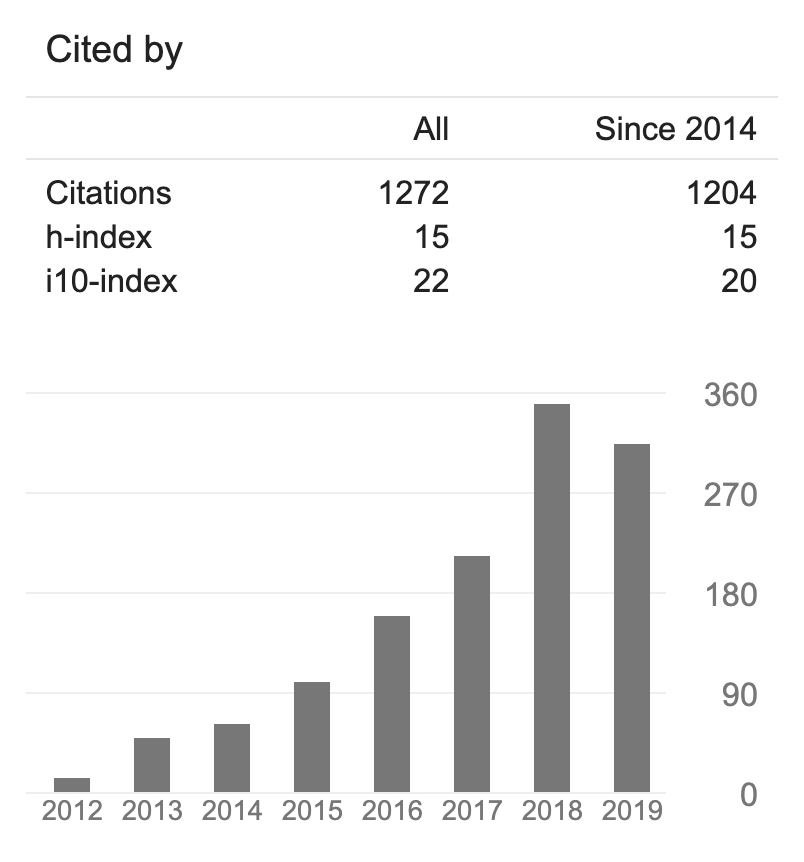
\includegraphics[width=60mm]{citation_091017.png}
  % \caption{Google Scholar Citations}
  % \label{fig:citation}
\end{figure}

\vspace{36pt}

{\centering \faCalendarCheckO~\today \par}

\end{document}
